%%%%%%%%%%%%%%%%%%%%%%%%%%%%%%%%%%%%%%%%%%%%%%%%%%%%%%%%%%%%%%%%%%%%%%%%%%%%%%%
%%
%% Copyright © 2022 Tropic Square s.r.o. (https://tropicsquare.com/)
%%
%% This work is subject to the license terms of the LICENSE.txt file in the
%% root directory of this source tree.
%%
%% If a copy of the LICENSE file was not distributed with this work, you can
%% obtain one at (https://tropicsquare.com/license).
%%
%%%%%%%%%%%%%%%%%%%%%%%%%%%%%%%%%%%%%%%%%%%%%%%%%%%%%%%%%%%%%%%%%%%%%%%%%%%%%%%
%
% This is user manual for Tropic Square Synthesis launch scrip.
%
% LaTex class:
%    tropic_design_spec
%
%%%%%%%%%%%%%%%%%%%%%%%%%%%%%%%%%%%%%%%%%%%%%%%%%%%%%%%%%%%%%%%%%%%%%%%%%%%%%%%
%%%%%%%%%%%%%%%%%%%%%%%%%%%%%%%%%%%%%%%%%%%%%%%%%%%%%%%%%%%%%%%%%%%%%%%%%%%%%%%

% Specify Tropic Square document class
\documentclass{tropic_design_spec}

% Code samples
\usepackage{listings}
\lstset{backgroundcolor=\color{lightgray}}

%%%%%%%%%%%%%%%%%%%%%%%%%%%%%%%%%%%%%%%%%%%%%%%%%%%%%%%%%%%%%%%%%%%%%%%%%%%%%%%
% Document properties and title page
%%%%%%%%%%%%%%%%%%%%%%%%%%%%%%%%%%%%%%%%%%%%%%%%%%%%%%%%%%%%%%%%%%%%%%%%%%%%%%%
\title{ts-hw-scripts: lint rtl flow - spyglass}
\author{Jan Zapeca, Tropic Square}
\date{October 2022}

% Start of document
\begin{document}

% Parameters Needed by Design spec class (must be inside document)
% Set these parameters according to your project.
\def \projectname {ts-hw-scripts: lint RTL flow}
\def \documentname {user guide}
\def \versionnumber {0.1}

% Title page
\maketitle


%%%%%%%%%%%%%%%%%%%%%%%%%%%%%%%%%%%%%%%%%%%%%%%%%%%%%%%%%%%%%%%%%%%%%%%%%%%%%%%
% Document revisions
% We revision with GIT, however, it does not mean that major changes in the
% document should not be kept also with document!
% In general, when you increase document version number, add also entry to
% this table with revisions saying what changed!
%%%%%%%%%%%%%%%%%%%%%%%%%%%%%%%%%%%%%%%%%%%%%%%%%%%%%%%%%%%%%%%%%%%%%%%%%%%%%%%
\section*{Version history}

\begin{TropicRatioLongTable4Col}
    {0.1}            {0.2}                {0.3}            {0.4}
    {Version Tag     & Date                 & Author        &    Description                    }
      0.1            & 20.4.2023            & Zapeca J.     &    Initial document version                   \Ttlb
\end{TropicRatioLongTable4Col}


%%%%%%%%%%%%%%%%%%%%%%%%%%%%%%%%%%%%%%%%%%%%%%%%%%%%%%%%%%%%%%%%%%%%%%%%%%%%%%%
% Table of contents
%%%%%%%%%%%%%%%%%%%%%%%%%%%%%%%%%%%%%%%%%%%%%%%%%%%%%%%%%%%%%%%%%%%%%%%%%%%%%%%
\pagebreak
\tableofcontents


%%%%%%%%%%%%%%%%%%%%%%%%%%%%%%%%%%%%%%%%%%%%%%%%%%%%%%%%%%%%%%%%%%%%%%%%%%%%%%%
%%%%%%%%%%%%%%%%%%%%%%%%%%%%%%%%%%%%%%%%%%%%%%%%%%%%%%%%%%%%%%%%%%%%%%%%%%%%%%%
% Document
%%%%%%%%%%%%%%%%%%%%%%%%%%%%%%%%%%%%%%%%%%%%%%%%%%%%%%%%%%%%%%%%%%%%%%%%%%%%%%%
%%%%%%%%%%%%%%%%%%%%%%%%%%%%%%%%%%%%%%%%%%%%%%%%%%%%%%%%%%%%%%%%%%%%%%%%%%%%%%%

%%%%%%%%%%%%%%%%%%%%%%%%%%%%%%%%%%%%%%%%%%%%%%%%%%%%%%%%%%%%%%%%%%%%%%%%%%%%%%%%%%%%%%%%%%%%%%%%%%%%
% Introduction
%%%%%%%%%%%%%%%%%%%%%%%%%%%%%%%%%%%%%%%%%%%%%%%%%%%%%%%%%%%%%%%%%%%%%%%%%%%%%%%%%%%%%%%%%%%%%%%%%%%%
\pagebreak
\TsSection{Introduction}

This document is a user guide for spyglass lint rtl flow that is part of ts-hw-scripts. The flow consists of:

\begin{itemize}
    \item \textit{ts_lint_rtl_run.py} Main script of the ts-hw-scripts lint rtl flow.
\end{itemize}

The spyglass lint rtl flow expects input files:

\begin{itemize}
    \item \textit{ts_sim_config.yml} Simulation config file specifying an RTL target and source lists
    \item \textit{ts_design_config.yml} Design config file specifying used IPs and design libraries
    \item \textit{ts_pdk_config.yml} PDK config file specifying available PDK
    \item \textit{rtl_<mode_name>.sgdc} Spyglass constraint file
\end{itemize}

The flow generates these files:

\begin{itemize}
    \item \textit{design_cfg.tcl} Auto-generated TCL script consists of available PDK digital views
    \item \textit{src_rtl.tcl} Auto-generated TCL script for sourcing RTL
    \item \textit{rtl_runfile.tcl} Auto-generated TCL script for opening an RTL lint results regarding selected runcode
\end{itemize}

Currently supported EDA tools:

\begin{itemize}
    \item \textit{SPYGLASS by Synopsys} 
\end{itemize}

Recommended literature:
\begin{itemize}
    \item \textit{Spyglass Base methodology} 
    \item \textit{Spyglass BuildInRules} 
    \item \textit{Spyglass ExplorerUsedGuide} 
    \item \textit{Spyglass TclShellInterfaceUserGuide} 
\end{itemize}


%%%%%%%%%%%%%%%%%%%%%%%%%%%%%%%%%%%%%%%%%%%%%%%%%%%%%%%%%%%%%%%%%%%%%%%%%%%%%%%
% Block diagram
%%%%%%%%%%%%%%%%%%%%%%%%%%%%%%%%%%%%%%%%%%%%%%%%%%%%%%%%%%%%%%%%%%%%%%%%%%%%%%%
\TsSection{User Manual}

\TsSubSection{Lint RTL flow usage model}

\begin{figure}[h]
    \centering
    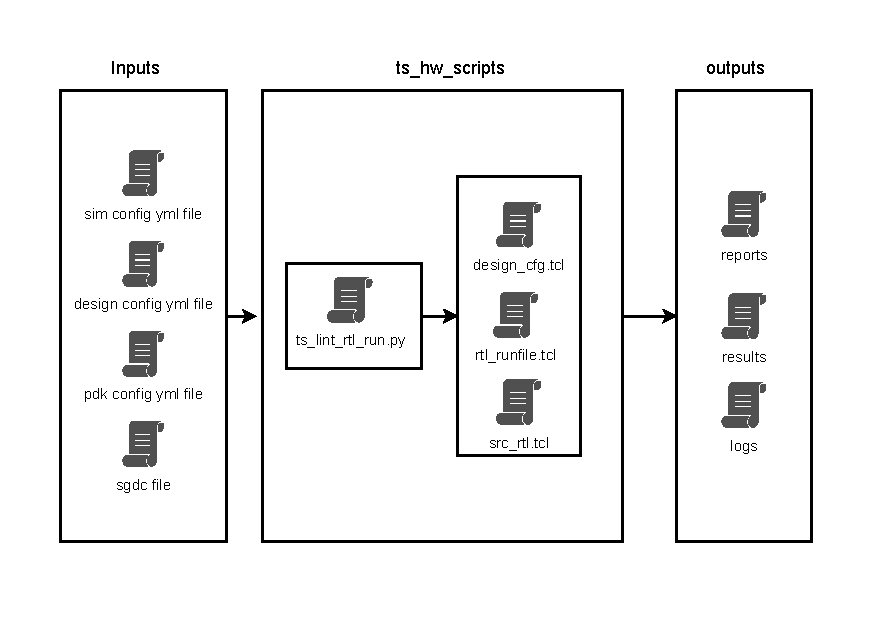
\includegraphics{%
        \detokenize{img/model.pdf}%
    }
    \caption{\projectname\space- usage model}
    \label{label}

\end{figure}


\TsSubSection{Command usage}

Execute a command to list all available features:

\begin{lstlisting}
    ts_lint_rtl_run.py --help
\end{lstlisting}

Execute a command to run a new lint rtl verification:

\begin{lstlisting}
    ts_lint_rtl_run.py --runcode <runcode> --mode <mode> --force --gui
\end{lstlisting}

Execute a command to open an rtl lint verification results:

\begin{lstlisting}
    ts_lint_rtl__run.py --runcode <runcode> --open-result --gui
\end{lstlisting}


\pagebreak

%%%%%%%%%%%%%%%%%%%%%%%%%%%%%%%%%%%%%%%%%%%%%%%%%%%%%%%%%%%%%%%%%%%%%%%%%%%%%%%
% Open issues
%%%%%%%%%%%%%%%%%%%%%%%%%%%%%%%%%%%%%%%%%%%%%%%%%%%%%%%%%%%%%%%%%%%%%%%%%%%%%%%
\TsSection{Open Issues}

\OpenIssue{The flow is not fully tested yet}

\PrintOpenIssueSummary

\end{document}
